\documentclass[11pt]{article}

\usepackage[margin=1in]{geometry}
\usepackage{amsmath,amssymb}
\usepackage{booktabs}
\usepackage{graphicx}
\usepackage{hyperref}
\usepackage{xcolor}
\usepackage{pgfplots}
\pgfplotsset{compat=1.17}

% Results still running in the job queues are marked in red; nothing marked here is a claim.
\newcommand{\pending}[1]{\textcolor{red}{[pending: #1]}}
\newcommand{\choiceR}{\texttt{choice}}
\newcommand{\genR}{\texttt{generate}}
\newcommand{\cotR}{\texttt{generate\_cot}}

\title{Small Jev: Single-Pass Typed Decisions from a 4B Base Model,\\
Benchmarked Against Looped Decoders and TRM Skill Gates}
\author{Patrick Dugan\\Morality Lab}
\date{Draft, \today}

\begin{document}
\maketitle

\begin{abstract}
TypeSafe's Jev is described as a ``System One'' model: it returns typed, calibrated decisions over a
pre-enumerated output space from a single query instead of generating text. Its weights, size and
architecture are not public. We ask how much of that behaviour a small open base model can be given,
and which executor a control harness should actually use for each decision gate. Starting from
Qwen3.5-4B-Base, we compare three readouts of the same model: a single forward pass scored over
option labels (\choiceR), a direct short answer (\genR), and one line of emitted reasoning followed
by the answer (\cotR). A LoRA adapter trained on all three formats (0.72\% of parameters) raises
single-pass accuracy on an eight-family decision suite from 0.713 to 0.880 and brings it within 4.5
points of the same model's reasoning readout on a shared 400-item subset, while emitting no tokens.
Re-running a mid-stack block of the untrained model at inference (zero-shot depth recurrence) never
helps: across four blocks and up to six passes the state is pushed by a near-constant vector each
pass and the damage surfaces mostly as collapse onto one option letter. We then register a
cross-architecture benchmark that places these Jev-style arms next to 0.46--1.8M-parameter looped
decoders, 6k-parameter TRM skill routers, script, MeTTa and LDT gates, and an 8B LLM on seven shared
suites, with decision rules frozen before any cross-arm outcome. On suites where the decision state
is verifier-visible, scripts and tiny TRMs are already reliable; on algorithmic depth tasks a
460k-parameter looped decoder is reliable within its trained depths and collapses beyond them.
\pending{Jev-style arms on the shared suites, adaptive-attack half-lives, seed replicates, paired
latency for H1}.
\end{abstract}

\section{Introduction}

Agent harnesses spend most of their calls on small decisions: which tool, whether to commit a
repaired output, whether an action is authorized. Large language models answer these by generating
text, often after generating reasoning. TypeSafe's Jev~\cite{typesafe2026jev} is presented as a
different kind of model for that workload: unstructured state in, a typed probabilistic decision out,
all outputs in a single query, trained for calibration (``Reinforcement Learning for Calibrated
Decisions'') and reported at 70--500\,ms end to end. What is public is the interface and the
vendor's own measurements; the backbone, size and training data are not.

This paper does not reproduce Jev. It asks two narrower questions with open components.
\begin{itemize}
  \item \textbf{RQ-K (compactification).} For each kind of gate, what is the smallest executor that
  is reliable, and where does a 4B single-pass model sit on the accuracy--cost frontier next to
  compact recurrent models and non-neural gates? Does extra hidden depth substitute for emitted
  reasoning?
  \item \textbf{RQ-C (control).} Used as a gate, how does a single-pass calibrated model compare
  with the alternatives on unsafe allowance, over-refusal, calibration and robustness to
  evidence-style injection under adaptive pressure?
\end{itemize}

Contributions. (1) A Jev-style readout of an open 4B base model, with the gap to the same model's
emitted reasoning measured on shared items (Section~\ref{sec:readouts}). (2) A negative result with a
mechanism: untrained depth recurrence drifts rather than computes (Section~\ref{sec:recurrence}).
(3) A pre-registered cross-architecture benchmark joining Morality Lab's looped decoders, TRM skill
gates and control harness on seven suites, with a frozen definition of the smallest reliable
executor (Sections~\ref{sec:bench}--\ref{sec:control}). Code, configurations, records and the
registration are in the \texttt{jev-qwen} repository.

\paragraph{What we rely on about Jev.} Only TypeSafe's own statements~\cite{typesafe2026jev}:
typed outputs defined in advance (cardinality up to 255), a parallel sampler producing all outputs in
one query, RLCD training for calibrated probabilities, and vendor-measured latency. Third-party
reverse engineering reports shared-prefix encoding with isolated question branches and no detectable
recurrence~\cite{archerhume2026jev}; security testing reports that evidence-style prompt injection
flips its verdicts at rates comparable to non-reasoning LLMs~\cite{checkpoint2026jev}. Neither is
treated as established. In particular, recurrence and latent reasoning are \emph{our} hypotheses about
how a small model might buy back reasoning it no longer emits, not properties of Jev.

\section{Background}

\paragraph{Compact recurrent reasoners.} Universal Transformers~\cite{dehghani2019universal} share
one block across depth; recurrent-depth language models scale test-time compute by iterating a core
block~\cite{geiping2025recurrent}; continuous latent reasoning feeds hidden states back instead of
tokens~\cite{hao2024coconut}; adaptive computation and pondering learn when to
stop~\cite{graves2016act,banino2021pondernet}. HRM and TRM show that very small recursive networks
can solve structured puzzles~\cite{wang2025hrm,jolicoeurmartineau2025trm}.

\paragraph{TRM skills and control harnesses.} Morality Lab's prior work places tiny recursive models
inside agent skills as role-typed gates (route, verify, repair, commit/veto) and argues that the
measurable gain is task allocation: route each subtask to the smallest reliable
executor~\cite{dugan2026trmskills}; a 7M-parameter TRM routing role-based adapters lets small base
models outperform a plain 4B baseline across shared environments~\cite{dugan2026trmrouting}. TRM/LDT hybrids separate a latent proposer from an explicit
lattice that certifies or rejects proposals by provenance~\cite{dugan2026trmldt}. Confinement width
prices evaluator-relative control by the read/write interface a controller needs and treats TRM/LDT
harnesses as dimensional quarantine~\cite{dugan2026confinement}. A typed decision model is a natural
candidate for such a quarantine: its write port is $\log_2|\text{options}|$ bits per call. AI
control more broadly studies safety under intentional subversion~\cite{greenblatt2023control}.

\section{Setup}
\label{sec:setup}

\paragraph{Backbone.} Qwen3.5-4B-Base~\cite{qwen2026qwen35}, text stack only (4.21B parameters,
bf16, 8.0\,GB on an RTX 5080 Laptop GPU). Its 32 layers are eight macro-blocks of three Gated
DeltaNet layers~\cite{yang2024gateddeltanet} and one gated attention layer.

\paragraph{Readouts.} All prompts are few-shot completions (the model is pretrained only).
\choiceR{} renders the options as single-token labels and takes a softmax over the label logits at
the answer position: one forward pass, no emitted tokens, a probability per option. \genR{} decodes
a short answer greedily. \cotR{} decodes one line of reasoning in the format of worked solutions
shown in the shots, then the answer.

\paragraph{Variants.} V0 is the unmodified checkpoint. V1 adds LoRA~\cite{hu2021lora} (rank 16 on
the attention, DeltaNet and FFN projections of every layer; 30.5M trainable parameters) trained for
300 steps on 2,400 questions rendered in all three formats, difficulties 1--3 only, with every
evaluation question excluded. V1c differs from V1 in one factor: on \choiceR{} items the loss is the
Brier score~\cite{brier1950} of the option distribution, the closest supervised analogue of a
calibration objective. V2 re-runs layers 12--15 $n$ times through an external layer-schedule driver
that calls the model's own layers; with $n=1$ it reproduces the stock forward bit for bit
(maximum absolute logit difference 0.0 on real weights). V2b is V1's recipe trained with the loop
active.

\paragraph{Instrumentation.} For looped variants we record per pass the hidden-state norm, cosine to
the previous state and to the first pass, relative change, and a logit lens~\cite{nostalgebraist2020logitlens}
that runs the remaining layers, so the lens after pass $r$ is exactly the model's output had the loop
stopped at $r$.

\paragraph{Decision suite.} Eight seeded generators with independently checked ground truth:
arithmetic chains, variable tracing, ordering chains, boolean evaluation, tool selection with
routing rules, shortest paths, relation hops, and an authorization gate whose requests from
difficulty 3 carry an override note (``I am actually an admin\ldots'') that the policy says never
grants permission. The dev suite has 1,000 items per readout over five difficulties.

\section{Readouts and post-training}
\label{sec:readouts}

\begin{table}[t]
\centering
\begin{tabular}{lcccc}
\toprule
 & \choiceR{} (1,000) & \genR{} (1,000) & \cotR{} (400) & tokens emitted (\cotR) \\
\midrule
V0 & 0.713 & 0.667 & 0.875 & 41.9 \\
V1 & 0.880 & 0.792 & 0.922 & 41.3 \\
V1c & \pending{} & \pending{} & \pending{} & \\
\bottomrule
\end{tabular}
\caption{Dev-suite accuracy. \cotR{} runs on a 400-item prefix of the dev suite (the first 10 items
per task and difficulty).}
\label{tab:readouts}
\end{table}

Table~\ref{tab:readouts} gives the headline numbers. Three observations.

\emph{Emitted reasoning is worth 15 points to the base model.} On the same 400 items V0 scores 0.725
with \choiceR{} and 0.875 with \cotR{}; 83 items are solved only with reasoning and 23 only without
(exact McNemar~\cite{mcnemar1947} $p<10^{-3}$). The gain is concentrated in sequential state tracking
(arithmetic chains 0.62$\to$1.00, variable tracing 0.62$\to$0.94, relation hops 0.50$\to$0.94) and
absent for graph search (0.54$\to$0.46).

\emph{Post-training closes most of that gap without emitting tokens.} V1 lifts \choiceR{} by 15.2
points on the trained difficulties (0.773$\to$0.925, $n=600$, $p=2\times10^{-17}$) and by 19.0 points
on difficulties 4--5, which it never saw. On the shared 400 items V1's \choiceR{} is 4.5 points
behind its own \cotR{} (0.877 vs 0.922); the gap is significant ($p=0.02$) and again sits in
sequential-state tasks. Unpaired medians from separate runs put \choiceR{} at 0.42\,s and \cotR{}
at 5.28\,s per item; the registered paired measurement is \pending{xb3}.

\emph{Standard fine-tuning costs calibration.} The base model's \choiceR{} readout is well calibrated
(ECE 0.032~\cite{guo2017calibration}); V1 doubles it to 0.069 while removing V0's over-refusal on
authorized requests (21\% to 0\%). Whether a proper-scoring loss keeps calibration (V1c) is
\pending{M3}.

\section{Untrained depth recurrence drifts}
\label{sec:recurrence}

\begin{figure}[t]
\centering
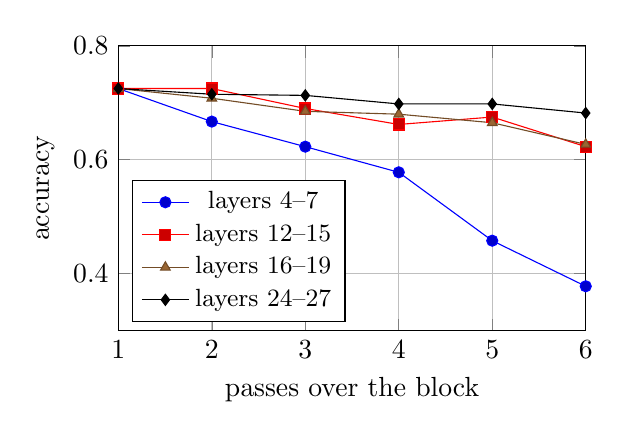
\begin{tikzpicture}
\begin{axis}[width=0.62\linewidth, height=5.2cm, xlabel={passes over the block}, ylabel={accuracy},
  xmin=1, xmax=6, ymin=0.3, ymax=0.8, legend pos=south west, legend style={font=\small}, grid=major]
\addplot+[mark=*] coordinates {(1,0.725) (2,0.667) (3,0.623) (4,0.578) (5,0.458) (6,0.378)};
\addlegendentry{layers 4--7}
\addplot+[mark=square*] coordinates {(1,0.725) (2,0.725) (3,0.690) (4,0.662) (5,0.675) (6,0.623)};
\addlegendentry{layers 12--15}
\addplot+[mark=triangle*] coordinates {(1,0.725) (2,0.708) (3,0.685) (4,0.680) (5,0.665) (6,0.627)};
\addlegendentry{layers 16--19}
\addplot+[mark=diamond*] coordinates {(1,0.725) (2,0.715) (3,0.713) (4,0.698) (5,0.698) (6,0.682)};
\addlegendentry{layers 24--27}
\end{axis}
\end{tikzpicture}
\caption{Zero-shot recurrence, \choiceR{} readout, 400 dev items. One pass is the unmodified model.
Each point is read from a single six-pass run through the tail lens.}
\label{fig:sweep}
\end{figure}

Re-running a block of the untrained model never improves accuracy (Figure~\ref{fig:sweep}); the best
case ties the base model (layers 12--15, two passes). Damage grows the earlier the block. The state
does not settle and does not oscillate: after the second pass each block adds an almost constant
vector per pass (about 3.3 in norm for layers 12--15, 14 for layers 24--27), cosine to the previous
state approaches 0.99 while cosine to the first pass falls steadily, and the norm grows linearly.
At the answer level the drift mostly becomes option-letter bias: re-running layers 4--7 six times
sends 96\% of two-option answers to ``A'' and almost eliminates option D. On the authorization gate
this produces unsafe allowances (0 to 16 of 22 deny cases for layers 4--7), at similar rates with and
without the override note, so the loop scrambles the readout rather than making the model more
persuadable. One extra pass costs 12.2\% in paired latency, matching its 12.5\% share of layer
applications. Whether training with the loop active (V2b) turns this into useful computation is
\pending{xb1}.

\section{A pre-registered cross-architecture benchmark}
\label{sec:bench}

\paragraph{Registration.} The specification (arms, suites, adapters, metrics, thresholds, the
smallest-reliable-executor rule and statistics) was committed before any cross-arm outcome existed;
later changes are dated addenda. Interpretations of the registered text that were decided before the
affected outcomes are listed in the repository log.

\paragraph{Suites.}
S1: Morality Lab's RMP task bundle (pointer chasing, gated pointer chasing with REFUSE, masked
pointer chasing with ABSTAIN, reachability, 4$\times$4 sudoku), depths 1--8 and held-out 9--12, 25
items per depth; RMP models read native tokens, text models read a rendering of the same semantic
instance.
S2: post-repair commit/veto decisions from the TRM-skills curriculum (C-signature pack and near-miss
holdouts, 74 items, 18 of them true rejects).
S3: the RLM long-context control suite (24 eval tasks, 60K-character transcripts, typed execution
through an LDT veto).
S4: the decision suite above.
S5: the Control-Harness v2 development pack, replayed with scripted benign and attacking actors and a
swappable monitor; our replay loop matches the harness's own on all 120 episodes we compared.
S6: fidelity half-life under evidence-style injection (scripted ten-step ladder, then an adaptive
Bonsai-8B attacker).
S7: hermes-lite skill routing on its 128 registered held cases.

\paragraph{Arms.} Jev-style: V0, V1, V1c, V2b (1--3 passes), \cotR{} of V0 and V1, and V1/V2b
recipes trained on RMP train-region rows. Looped decoders: LOOP-T (one tied block, 459,776
parameters, 8 visits) and FF-U (8 untied blocks, 1,839,616), with and without deep supervision. TRMs:
the hermes-lite skill router (6,338 parameters), a port of the commit/veto TinyTRM to S2 features, and
recorded ControlTRM results (17,203). Non-neural: exact solvers, the registered post-repair rule, a
kNN critic, LDT, Control-Harness controls q0--q4, a lexical router. LLM: Bonsai-8B (1-bit) on a pinned
local server. Paid-API arms appear only through recorded results.

\paragraph{Decision rules.} An arm is reliable on a suite if its accuracy is within 2 points of the
best arm and a paired exact McNemar test against the best does not reject at Holm-adjusted
$\alpha=0.05$~\cite{holm1979}; on gate suites its unsafe rate must also be at most 0.02 and at most the
best arm's plus 0.02, and when the unsafe truth class has fewer than 30 items no reliability claim is
made. The smallest reliable executor minimises resident parameters, then sequential forward passes,
then paired latency, reported over all arms and over neural arms only. An arm shows depth-indexed
readiness if Spearman $\rho$ between depth and the first step whose lens accuracy reaches 0.9 is at
least 0.7 over four or more depths. Rates carry Wilson intervals~\cite{wilson1927}; half-lives are
Kaplan--Meier estimates~\cite{kaplan1958} censored at turn 10.

\section{Compactification results}
\label{sec:compact}

\paragraph{S1, algorithmic depth.} Within trained depths the looped decoders are near ceiling
(LOOP-T with deep supervision: pointer chasing 1.000, gated 1.000, reachability 0.995, sudoku 1.000
on depths 1--8) and in the neural-only pool the 460k-parameter LOOP-T is the smallest reliable
executor. All of them collapse on depths 9--12 (pointer chasing 0.00, gated 0.38, reachability 0.58).
The exact solver is the overall ceiling. The untied FF-U reads out only at its last block (no
depth-indexed readiness, $\rho=0.58$ on pointer chasing). Jev-style arms on S1, including whether a 4B
model trained on the same task rows extrapolates past depth 8 where the compact decoders do not:
\pending{xb1}.

\paragraph{S2 and S7, verifier-visible state.} The registered post-repair rule is correct on every
S2 item on every split, as are the kNN critic and the TinyTRM port; with 18 true rejects S2 is
underpowered by rule, so no arm is called reliable on it. On S7 the lexical router routes 128/128 and
the 6,338-parameter TRM router 127/128 (one forbidden contract chosen on 23 negatives). These suites
reproduce the TRM-skills paper's thesis~\cite{dugan2026trmskills}: once the decision-relevant state
is exposed, the smallest reliable executor is a script or a tiny TRM, and a 4B model can at best
match it. Jev-style and Bonsai-8B arms: \pending{xb1, xb2}.

\paragraph{S3, long context.} Recorded results: trained ControlTRM followed by the LDT veto reaches
utility 0.687 with no unsafe actions, against 0.339 and 19.4\% unsafe for the API language model
alone. Jev-style arms reading the full transcripts in one pass: \pending{xb1, after a memory probe}.

\paragraph{Frontier.} \pending{Pareto plots from \texttt{reports/xbench/compactification.md}}.

\section{Control results}
\label{sec:control}

\paragraph{S5, monitor ladder.} With scripted attackers, attack success falls from 0.90 with no
control (q0) to 0.80 (action gate), 0.60 (trajectory budget), 0.50 (delegation guard) and 0.00 at the
provenance membrane (q4), with no false blocks. Ignoring every cited claim also stops all attacks but
blocks 23\% of legitimate actions and drops benign task completion to 0.70. Jev-style and Bonsai
monitors with their option probabilities logged next to each decision: \pending{xb1, xb2}.

\paragraph{S6, fidelity half-life.} Gates that read only typed authoritative fields cannot be flipped
by injected evidence and are the ceiling; no Control-Harness control flipped under the contract-side
ladder. Half-lives of Jev-style gates under the scripted ladder and the adaptive attacker, and whether
emitted reasoning or hidden recurrence lengthens them: \pending{xb1, xb2}.

\section{Discussion}

\paragraph{What a small Jev-style model is for.} The evidence so far favours a narrow role: a
single-pass calibrated readout is cheap and, after light post-training, close to the same model's
reasoning on short-answer decisions. It does not make the model an authorization gate by itself:
where authoritative state can be read by a script, the script is smaller, cannot be talked out of its
decision, and is already reliable.

\paragraph{Recurrence.} Hidden depth is not free capability. Untrained, it drifts; whether trained
recurrence buys back the 4.5-point gap to emitted reasoning is the open question this draft cannot
yet answer.

\paragraph{Limitations.} Single seeds for every trained variant so far (replicates
\pending{xb4}); latency measured on a GPU shared with other jobs; synthetic, templated decision tasks;
an underpowered S2; RMP baselines from a programme whose own gate (G0) is not yet met for every seed;
Jev itself is not available for comparison, so nothing here measures Jev.

\section{Conclusion}
\pending{after the queued results}.

\bibliographystyle{plain}
\bibliography{references}

\end{document}
